% --- IMPORTS ---
\documentclass[leqno]{article}
\usepackage{graphicx}
\usepackage{dsfont}
\usepackage{mathtools}
\usepackage{amssymb}
\usepackage{amsmath}
\usepackage{amsthm}
\usepackage{float}
\usepackage{ragged2e}
\usepackage{tensor}
\usepackage{fancyhdr}
\usepackage{empheq}
\usepackage[most]{tcolorbox}
\usepackage{enumitem}
\usepackage{dirtytalk}
\usepackage{marginnote}
\usepackage{microtype}
\usepackage[
  a4paper,
  left=0.8in,
  right=1in,
  top=1in,
  bottom=0.5in,
  headheight=14pt,
  headsep=0.4in
]{geometry}
\setlength{\parindent}{0cm}
% --- TikZ Packages ---
\usepackage{pgfplots}
\pgfplotsset{compat=1.18}
\usepgfplotslibrary{fillbetween, polar}
\usetikzlibrary{calc, positioning}
\usetikzlibrary{angles, quotes}
\usetikzlibrary{arrows.meta}
\usetikzlibrary{decorations.pathreplacing, decorations.markings}
\usetikzlibrary{patterns}
\usetikzlibrary{intersections}
% --- URL Packages ---
\usepackage[colorlinks=true,linkcolor=red,citecolor=magenta,urlcolor=black]{hyperref}%
\urlstyle{same}
% --- END OF IMPORTS ---

% --- CUSTOM COMMANDS ---
\RenewDocumentCommand{\marks}{o m}{%
  \IfValueTF{#1}%
    {\marginnote{\raggedright\textbf{[#2]}}[#1]}%
    {\marginnote{\raggedright\textbf{[#2]}}}%
}
\newcommand{\vspacerule}[2]{%
  \par\vspace*{#1}%
  \noindent\hrulefill\par
  \vspace*{#2}%
}
\definecolor{scarlet}{RGB}{205, 40, 75}
\newcommand{\questionitem}{%
  \item\phantomsection
  \addcontentsline{toc}{section}{Question \number\value{enumi}}%
}
\renewcommand{\contentsname}{Questions}
% --- END OF CUSTOM COMMANDS ---

% --- HEADER CONFIG ---
\pagestyle{fancy}
\fancyhead{}
\fancyfoot{}
\renewcommand{\headrulewidth}{0.9pt}
\lhead{\textit{Solutions} - Loci and Regions in the Argand Diagram}
\chead{}
\rhead{\href{https://danieljsmith.org}{danieljsmith.org}}
% --- END OF HEADER CONFIG ---

\begin{document}
\vspace*{20pt}
\tableofcontents
\newpage
\begin{enumerate}[
  label=\textbf{\arabic*.},
  leftmargin=*,
  topsep=0pt,
  partopsep=0pt,
  parsep=0pt
]

% ---- Question 1 ----
\questionitem

\begin{figure}[H]
    \centering
\begin{tikzpicture}[scale=0.75]
\def\cx{-2}
\def\cy{1}
\def\rad{4}

\coordinate (C) at (\cx,\cy);

\draw[-{Stealth[length=3mm]}, thick] (-6.3,0) -- (4.7,0) node[right] {$\mathrm{Re}(z)$};
\draw[-{Stealth[length=3mm]}, thick] (0,-4.3) -- (0,6.3) node[above] {$\mathrm{Im}(z)$};

\draw[thick] (C) circle (\rad);

\draw[thick] (\cx,0.12) -- (\cx,-0.12);
\draw[thick] (0.12,\cy) -- (-0.12,\cy);

\node[below left] at (0,0) {$O$};
\node[below] at (\cx,0) {$-2$};
\node[left] at (0,\cy) {$1$};
\end{tikzpicture}
\end{figure}


The Argand diagram shows a circle of radius $4$. The centre of the circle is the point which represents the complex number $-2+\mathrm{i}$. \\

\begin{enumerate}[label=\textbf{(\alph*)}]
  \item Use set notation to define the locus of complex numbers, $z$, represented by points which lie on the circle. \marks{2} \\
\end{enumerate}

The locus $L$ is defined by
\[
L=\Bigl\{z\in\mathbb{C}\;\Bigm|\; |z-(-2+\mathrm{i})|=|z+1-3\mathrm{i}|\Bigr\}
\] \\

\begin{enumerate}[label=\textbf{(\alph*)}, resume]
  \item On a copy of the Argand diagram, sketch and label the locus $L$. \marks{2} \\
\end{enumerate}

You are given that the locus
\[
\Bigl\{z\in\mathbb{C}\;\Bigm|\; \arg(z+1-2\mathrm{i})=\frac{2\pi}{3},\ \mathrm{Im}(z)=5\Bigr\}
\]
contains only one number. \\

\begin{enumerate}[label=\textbf{(\alph*)}, resume]
  \item Find this number. \marks{2} \\
\end{enumerate}

\vspace*{10pt}

\begin{tcolorbox}[colback=white, colframe=scarlet, title={\textbf{Solution}}, breakable, grow to left by=6mm, grow to right by=10mm]
\begin{enumerate}[label=\textbf{(\alph*)}]
  \item The circle has centre \(-2+\mathrm{i}\) and radius \(4\).

So the locus is the set of complex numbers whose distance from \(-2+\mathrm{i}\) is \(4\):
\[
\{z\in\mathbb{C}\mid |z-(-2+\mathrm{i})|=4\}
=
\{z\in\mathbb{C}\mid |z+2-\mathrm{i}|=4\}
\]

Hence the locus is \(\{z\in\mathbb{C}\mid |z+2-\mathrm{i}|=4\}\).

  \item Let \(z=x+\mathrm{i}y\), where \(x,y\in\mathbb{R}\).

Then
\[
|z-(2+\mathrm{i})|=|z+1-3\mathrm{i}|
\]
gives
\[
|(x-2)+\mathrm{i}(y-1)|=|(x+1)+\mathrm{i}(y-3)|
\]

Squaring both sides:
\[
(x-2)^2+(y-1)^2=(x+1)^2+(y-3)^2
\]

Now expand:
\begin{align*}
x^2-4x+4+y^2-2y+1&=x^2+2x+1+y^2-6y+9\\
-4x-2y+5&=2x-6y+10\\
-6x+4y-5&=0\\
6x-4y+5&=0
\end{align*}

So
\[
L:\ 6x-4y+5=0
\]
or equivalently
\[
y=\frac{3}{2}x+\frac{5}{4}
\]

This is a straight line. Since it is the set of points equidistant from \(2+\mathrm{i}\) and \(-1+3\mathrm{i}\), it is the perpendicular bisector of the line segment joining those two points.

Its midpoint is
\[
\left(\frac{2+(-1)}{2},\frac{1+3}{2}\right)=\left(\frac12,2\right)
\]

\begin{figure}[H]
    \centering
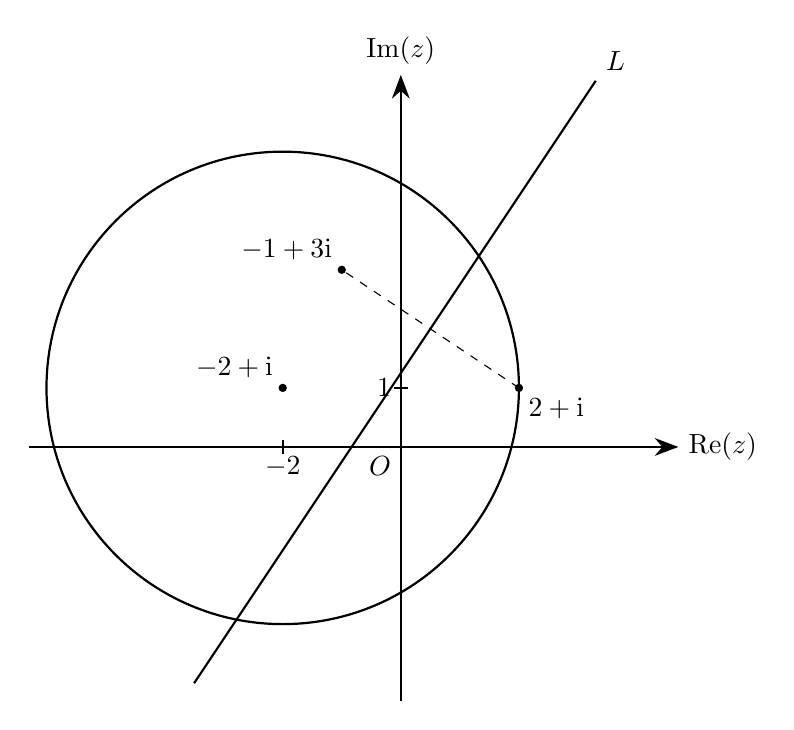
\begin{tikzpicture}[scale=0.75]
\def\xmin{-6.3}
\def\xmax{4.7}
\def\ymin{-4.3}
\def\ymax{6.3}
\def\cx{-2}
\def\cy{1}
\def\rad{4}

\coordinate (O) at (0,0);
\coordinate (C) at (-2,1);
\coordinate (A) at (2,1);
\coordinate (B) at (-1,3);

\draw[-{Stealth[length=3mm]}, thick] (\xmin,0) -- (\xmax,0) node[right] {$\mathrm{Re}(z)$};
\draw[-{Stealth[length=3mm]}, thick] (0,\ymin) -- (0,\ymax) node[above] {$\mathrm{Im}(z)$};

\draw[thick] (C) circle (\rad);

\draw[thick] (-3.5,-4) -- (3.3,6.2) node[above right] {$L$};

\draw[dashed] (A) -- (B);

\fill (C) circle (2pt);
\fill (A) circle (2pt);
\fill (B) circle (2pt);

\draw[thick] (\cx,0.12) -- (\cx,-0.12);
\draw[thick] (0.12,\cy) -- (-0.12,\cy);

\node[below left] at (O) {$O$};
\node[below] at (\cx,0) {$-2$};
\node[left] at (0,\cy) {$1$};

\node[above left] at (C) {$-2+\mathrm{i}$};
\node[below right] at (A) {$2+\mathrm{i}$};
\node[above left] at (B) {$-1+3\mathrm{i}$};
\end{tikzpicture}
\end{figure}


  \item Since \(\mathrm{Im}(z)=5\), write
\[
z=x+5\mathrm{i}
\]

Then
\[
z+1-2\mathrm{i}=(x+1)+3\mathrm{i}
\]

We are given
\[
\arg(z+1-2\mathrm{i})=\frac{2\pi}{3}
\]

So the argument of \((x+1)+3\mathrm{i}\) is \(120^\circ\), which is in the second quadrant. Therefore
\[
\tan\frac{2\pi}{3}=\frac{3}{x+1}
\]

Using \(\tan\frac{2\pi}{3}=-\sqrt{3}\),
\[
\frac{3}{x+1}=-\sqrt{3}
\]

Hence
\[
x+1=-\sqrt{3}
\]
so
\[
x=-1-\sqrt{3}
\]

Therefore
\[
z=-1-\sqrt{3}+5\mathrm{i}
\]

So the required number is \(-1-\sqrt{3}+5\mathrm{i}\).
\end{enumerate}
\end{tcolorbox}


\newpage

% ---- Question 2 ----
\questionitem

In an Argand diagram, the point $P$ representing the complex number $w$ lies on the locus defined by \[\Bigl\{ z\in\mathbb{C}\;\Bigm|\; \arg(z-2+\mathrm{i})=\frac{\pi}{6} \Bigr\}\] You are given that $\mathrm{Im}(w)=3$. \\

\begin{enumerate}[label=\textbf{(\alph*)}]
  \item Find $w$. \marks{2} \\
\end{enumerate}

The point $P$ also lies on the locus defined by $\Bigl\{ z\in\mathbb{C}\;\Bigm|\; \lvert z-2-11\mathrm{i}\rvert =k \Bigr\}$, where $k$ is a constant. \\

\begin{enumerate}[label=\textbf{(\alph*)}, resume]
  \item Find the complex number represented by the other point of intersection of the loci defined by \[\Bigl\{ z\in\mathbb{C}\;\Bigm|\; \lvert z-2-11\mathrm{i}\rvert =k \Bigr\}\quad\text{and}\quad\Bigl\{ z\in\mathbb{C}\;\Bigm|\; \arg(z-2+\mathrm{i})=\frac{\pi}{6} \Bigr\}\] \marks{7} \\
\end{enumerate}

\vspace*{10pt}

\begin{tcolorbox}[colback=white, colframe=scarlet, title={\textbf{Solution}}, breakable, grow to left by=6mm, grow to right by=10mm]
\begin{enumerate}[label=\textbf{(\alph*)}]
  \item Let
  \[
  w=x+3\mathrm{i}
  \]
  since $\mathrm{Im}(w)=3$.

  Then
  \[
  w-2+\mathrm{i}=(x-2)+4\mathrm{i}
  \]

  Given
  \[
  \arg(w-2+\mathrm{i})=\frac{\pi}{6}
  \]
  so
  \[
  \tan\frac{\pi}{6}=\frac{4}{x-2}
  \]

  Hence
  \[
  \frac{1}{\sqrt{3}}=\frac{4}{x-2}
  \]
  so
  \[
  x-2=4\sqrt{3}
  \]
  and therefore
  \[
  x=2+4\sqrt{3}
  \]

  Thus
  \[
  w=2+4\sqrt{3}+3\mathrm{i}
  \]

  So the required complex number is $2+4\sqrt{3}+3\mathrm{i}$.

  \item From part (a),
  \[
  P \text{ represents } w=2+4\sqrt{3}+3\mathrm{i}
  \]

  The second locus is
  \[
  \lvert z-2-11\mathrm{i}\rvert=k=\lvert z-(2+11\mathrm{i})\rvert
  \]
  which is a circle with centre $2+11\mathrm{i}$.

  Using the point $P$ to find $k$,
  \begin{align*}
  k&=\left|w-(2+11\mathrm{i})\right| \\
   &=\left|(2+4\sqrt{3}+3\mathrm{i})-(2+11\mathrm{i})\right| \\
   &=\left|4\sqrt{3}-8\mathrm{i}\right|
  \end{align*}

  So
  \begin{align*}
  k^2&=(4\sqrt{3})^2+(-8)^2 \\
     &=48+64 \\
     &=112
  \end{align*}
  and hence
  \[
  k=4\sqrt{7}
  \]

  Now let a general point of intersection be
  \[
  z=x+y\mathrm{i}
  \]

  Since
  \[
  \arg(z-2+\mathrm{i})=\frac{\pi}{6}
  \]
  the point lies on the half-line starting at $(2,-1)$ with gradient
  \[
  \tan\frac{\pi}{6}=\frac{1}{\sqrt{3}}
  \]
  so its equation is
  \[
  y+1=\frac{x-2}{\sqrt{3}}
  \]
  that is,
  \[
  y=\frac{x-2}{\sqrt{3}}-1
  \]

  The circle has equation
  \[
  (x-2)^2+(y-11)^2=112
  \]

  Substitute $y=\dfrac{x-2}{\sqrt{3}}-1$:
  \[
  (x-2)^2+\left(\frac{x-2}{\sqrt{3}}-12\right)^2=112
  \]

  Let
  \[
  u=x-2
  \]
  Then
  \[
  u^2+\left(\frac{u}{\sqrt{3}}-12\right)^2=112
  \]

  Expanding,
  \begin{align*}
  u^2+\left(\frac{u^2}{3}-8\sqrt{3}\,u+144\right)&=112 \\
  \frac{4u^2}{3}-8\sqrt{3}\,u+144&=112 \\
  \frac{4u^2}{3}-8\sqrt{3}\,u+32&=0
  \end{align*}

  Multiply by $3$:
  \[
  4u^2-24\sqrt{3}\,u+96=0
  \]

  Divide by $4$:
  \[
  u^2-6\sqrt{3}\,u+24=0
  \]

  Factorising,
  \[
  (u-4\sqrt{3})(u-2\sqrt{3})=0
  \]

  So
  \[
  u=4\sqrt{3}\quad \text{or}\quad u=2\sqrt{3}
  \]

  The value $u=4\sqrt{3}$ gives the known point $P$ from part (a), so the other intersection has
  \[
  u=2\sqrt{3}
  \]

  Therefore
  \[
  x=2+2\sqrt{3}
  \]
  and
  \[
  y=\frac{2\sqrt{3}}{\sqrt{3}}-1=2-1=1
  \]

  Hence the other point represents
  \[
  z=2+2\sqrt{3}+\mathrm{i}
  \]

  So the other complex number is $2+2\sqrt{3}+\mathrm{i}$.
\end{enumerate}
\end{tcolorbox}


\newpage

% ---- Question 3 ----
\questionitem

On an Argand diagram, the locus of points satisfying $|z-4+3\mathrm{i}|=8$ is a circle. \\

\begin{enumerate}[label=\textbf{(\alph*)}]
  \item Write down
  \begin{enumerate}[label=(\roman*)]
    \item the coordinates of the centre of this circle \marks{1}
    \item the radius of this circle \marks{1}
  \end{enumerate}
  \item On an Argand diagram, shade the set of points defined by
  \[
  |z-4+3\mathrm{i}|\le 8
  \]
  \marks[-20pt]{1}
  \item For the set of points defined in part (b), determine the maximum value of $|z|$. \marks{3} \\
\end{enumerate}

The set of points $A$ is defined by
\[
A=
\Bigl\{ z\in\mathbb{C}\;\Bigm|\; -\frac{\pi}{4}\le \arg(z-3-6\mathrm{i})\le \frac{3\pi}{4} \Bigr\}
\mathbin{\textstyle\bigcap}
\Bigl\{ z\in\mathbb{C}\;\Bigm|\; \lvert z-4+3\mathrm{i}\rvert \le 8 \Bigr\}
\]

\begin{enumerate}[label=\textbf{(\alph*)}, resume]
  \item Determine the area of the region defined by $A$, giving your answer to 3 significant figures. \marks{4} \\
\end{enumerate}

\vspace*{10pt}

\begin{tcolorbox}[colback=white, colframe=scarlet, title={\textbf{Solution}}, breakable, grow to left by=6mm, grow to right by=10mm]
\begin{enumerate}[label=\textbf{(\alph*)}]
  \item
  \begin{enumerate}[label=(\roman*)]
    \item
    \[
    |z-4+3\mathrm{i}|=|z-(4-3\mathrm{i})|
    \]
    So the circle has centre \((4,-3)\).

    \item
    Comparing with the standard form \(|z-a|=r\), the radius is \(8\).
  \end{enumerate}

  \item
  The inequality
  \[
  |z-4+3\mathrm{i}|\le 8
  \]
  means all points whose distance from \(4-3\mathrm{i}\) is at most \(8\).

  So we shade the interior and boundary of the circle with centre \((4,-3)\) and radius \(8\).

  \begin{center}
  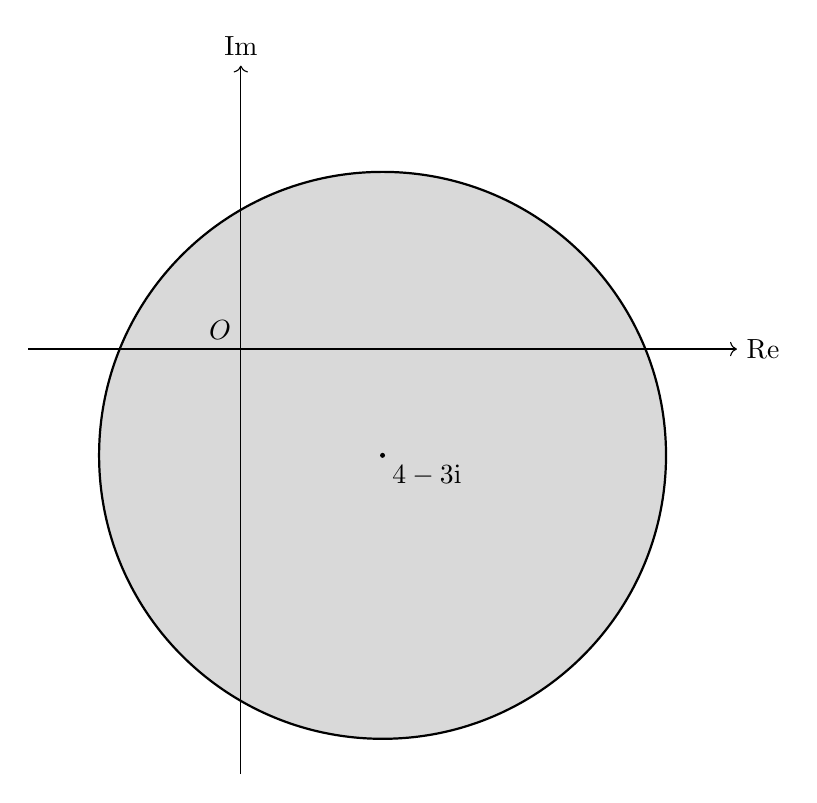
\begin{tikzpicture}[scale=0.45]
    \def\cx{4}
    \def\cy{-3}
    \def\rad{8}
    \fill[gray!30] (\cx,\cy) circle (\rad);
    \draw[->] (-6,0) -- (14,0) node[right] {Re};
    \draw[->] (0,-12) -- (0,8) node[above] {Im};
    \node[above left] at (0,0) {$O$};
    \draw[thick] (\cx,\cy) circle (\rad);
    \fill (\cx,\cy) circle (2pt);
    \node[below right] at (\cx,\cy) {$4-3\mathrm{i}$};
  \end{tikzpicture}
  \end{center}

  \item
  The modulus \(|z|\) is the distance from the origin.

  For any point in the region,
  \begin{align*}
  |z|
  &= |(z-4+3\mathrm{i})+(4-3\mathrm{i})| \\
  &\le |z-4+3\mathrm{i}|+|4-3\mathrm{i}| \\
  &\le 8+\sqrt{4^2+(-3)^2} \\
  &= 8+5 \\
  &= 13
  \end{align*}

  Equality is possible at the point on the circle lying on the line from the origin through the centre.

  Therefore the maximum value of \(|z|\) is \(13\).

  \item
  Let \(z=x+\mathrm{i}y\).

  First consider the argument condition:
  \[
  -\frac{\pi}{4}\le \arg(z-3-6\mathrm{i})\le \frac{3\pi}{4}
  \]

  Since
  \[
  z-3-6\mathrm{i}=(x-3)+\mathrm{i}(y-6)
  \]
  the boundary arguments \(-\pi/4\) and \(3\pi/4\) are opposite directions, so they form a straight line through \((3,6)\) with gradient \(-1\).

  Hence the boundary line is
  \[
  y-6=-(x-3)
  \]
  so
  \[
  x+y=9
  \]

  To decide which side is needed, take the point \((3,7)\). Then
  \[
  \arg\bigl((3+7\mathrm{i})-3-6\mathrm{i}\bigr)=\arg(\mathrm{i})=\frac{\pi}{2}
  \]
  which is in the given range, and \((3,7)\) satisfies \(x+y=10\).

  So the argument condition is the half-plane
  \[
  x+y\ge 9
  \]

  The circle has centre \(C=(4,-3)\) and radius \(8\). Since
  \[
  4+(-3)=1<9
  \]
  the centre lies on the opposite side of the line, so the region \(A\) is the minor segment cut off by the line \(x+y=9\).

  The perpendicular distance from \(C\) to the line \(x+y=9\) is
  \[
  d=\frac{|4+(-3)-9|}{\sqrt{1^2+1^2}}
   =\frac{8}{\sqrt{2}}
   =4\sqrt{2}
  \]

  Let \(P\) and \(Q\) be the points where the line meets the circle, and let \(M\) be the midpoint of chord \(PQ\). Then \(CM\perp PQ\), so in right-angled triangle \(CMP\),
  \[
  \cos \angle PCM=\frac{CM}{CP}=\frac{4\sqrt{2}}{8}=\frac{\sqrt{2}}{2}
  \]
  Hence
  \[
  \angle PCM=\frac{\pi}{4}
  \]
  so the angle subtended by the chord is
  \[
  \angle PCQ=2\times \frac{\pi}{4}=\frac{\pi}{2}
  \]

  Therefore
  \begin{align*}
  \text{Area}(A)
  &= \text{area of sector }PCQ-\text{area of }\triangle PCQ \\
  &= \frac12 r^2\theta-\frac12 r^2\sin\theta \\
  &= \frac12 \cdot 8^2 \cdot \frac{\pi}{2}-\frac12 \cdot 8^2 \cdot \sin\frac{\pi}{2} \\
  &= 16\pi-32
  \end{align*}

  So the area is
  \[
  16\pi-32 \approx 18.3
  \]
  to 3 significant figures.
\end{enumerate}
\end{tcolorbox}


\newpage

% ---- Question 4 ----
\questionitem

\begin{figure}[H]
    \centering
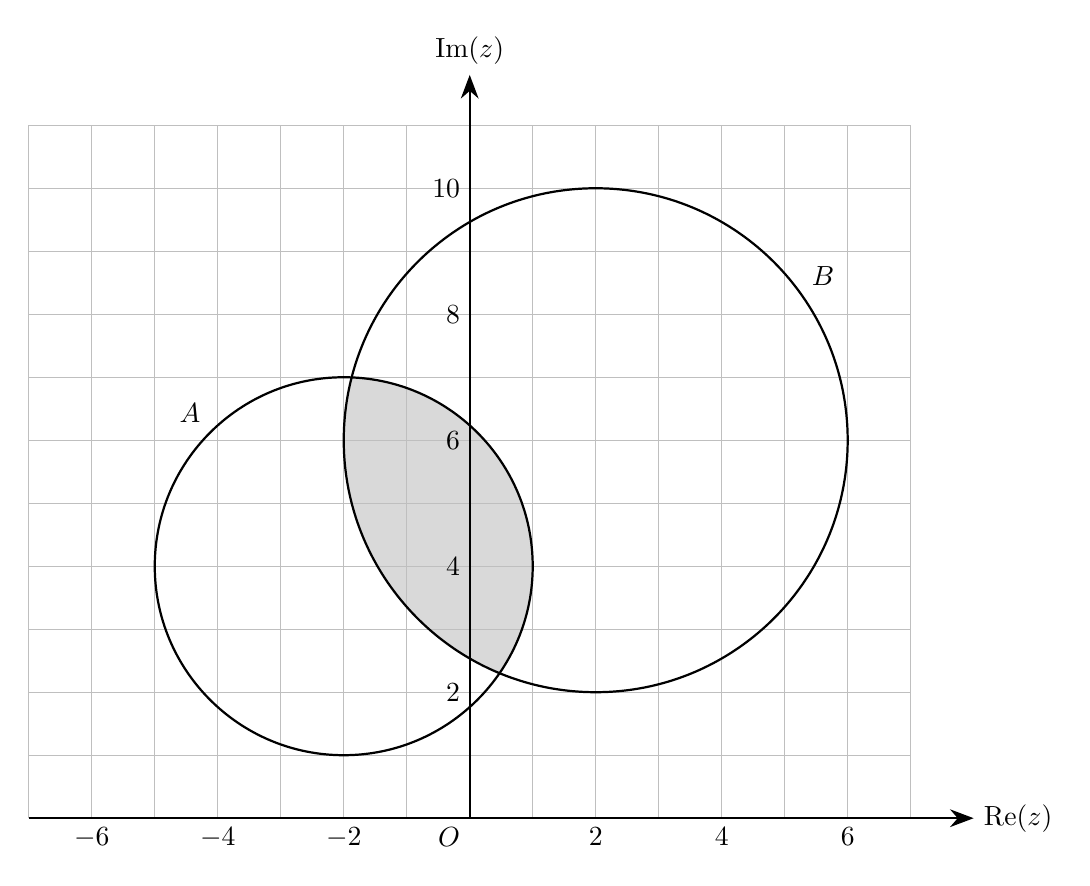
\begin{tikzpicture}[scale=0.8]
\def\xmin{-7}
\def\xmax{7}
\def\ymin{0}
\def\ymax{11}
\def\XA{-2}
\def\YA{4}
\def\RA{3}
\def\XB{2}
\def\YB{6}
\def\RB{4}

\coordinate (Ac) at (\XA,\YA);
\coordinate (Bc) at (\XB,\YB);

\begin{scope}
  \clip (Ac) circle (\RA);
  \fill[gray!30] (Bc) circle (\RB);
\end{scope}

\draw[gray!50, very thin] (\xmin,\ymin) grid (\xmax,\ymax);

\draw[thick] (Ac) circle (\RA);
\draw[thick] (Bc) circle (\RB);

\draw[-{Stealth[length=3mm]}, thick] (\xmin,0) -- (\xmax+1.0,0) node[right] {$\mathrm{Re}(z)$};
\draw[-{Stealth[length=3mm]}, thick] (0,\ymin) -- (0,\ymax+0.8) node[above] {$\mathrm{Im}(z)$};

\foreach \x in {-6,-4,-2,2,4,6} {
  \node[below] at (\x,0) {$\x$};
}
\foreach \y in {2,4,6,8,10} {
  \node[left] at (0,\y) {$\y$};
}
\node[below left] at (0,0) {$O$};

\node[above left] at ($(Ac)+(135:\RA)$) {$A$};
\node[above right] at ($(Bc)+(35:\RB)$) {$B$};
\end{tikzpicture}
\end{figure}


\begin{enumerate}[label=\textbf{(\alph*)}]
  \item The diagram above shows an Argand diagram.
  \begin{enumerate}[label=(\roman*)]
    \item Write down the equation of the locus represented by the circumference of circle $A$. \marks{3}
    \item Write down the two inequalities that define the shaded region, not including either circumference. \marks{3} \\
  \end{enumerate}
  \item
  \begin{enumerate}[label=(\roman*)]
    \item Draw an Argand diagram to show the region where
    \[
    -\frac{\pi}{6}<\arg\bigl(z+2-\mathrm{i}\bigr)<\frac{\pi}{4}
    \]
    \marks[-20pt]{3}
    \item Determine whether the point $1+5\mathrm{i}$ lies within this region. \marks{3} \\
  \end{enumerate}
\end{enumerate}

\vspace*{10pt}

\begin{tcolorbox}[colback=white, colframe=scarlet, title={\textbf{Solution}}, breakable, grow to left by=6mm, grow to right by=10mm]
\begin{enumerate}[label=\textbf{(\alph*)}]
  \item \begin{enumerate}[label=(\roman*)]
    \item For a circle with centre $z_0$ and radius $r$, the locus is
    \[
    |z-z_0|=r
    \]
    Circle $A$ has centre $-2+4\mathrm{i}$ and radius $3$, so
    \[
    |z-(-2+4\mathrm{i})|=3
    \]
    hence
    \[
    |z+2-4\mathrm{i}|=3
    \]
    So the equation of the circumference of circle $A$ is $|z+2-4\mathrm{i}|=3$.

    \item The shaded region is the part inside both circles, and neither circumference is included.

    Inside circle $A$:
    \[
    |z+2-4\mathrm{i}|<3
    \]

    Circle $B$ has centre $2+6\mathrm{i}$ and radius $4$, so inside circle $B$:
    \[
    |z-(2+6\mathrm{i})|<4
    \]

    So the two inequalities are
    \[
    |z+2-4\mathrm{i}|<3
    \qquad \text{and} \qquad
    |z-(2+6\mathrm{i})|<4
    \]
  \end{enumerate}

  \item \begin{enumerate}[label=(\roman*)]
    \item We have
    \[
    z+2-\mathrm{i}=z-(-2+\mathrm{i})
    \]
    so the argument is measured from the point $-2+\mathrm{i}$.

    The region
    \[
    -\frac{\pi}{6}<\arg(z+2-\mathrm{i})<\frac{\pi}{4}
    \]
    is therefore the open sector with vertex at $-2+\mathrm{i}$ between the rays making angles $-\frac{\pi}{6}$ and $\frac{\pi}{4}$ with the positive real axis.

    Since the inequalities are strict, both boundary rays are excluded.

    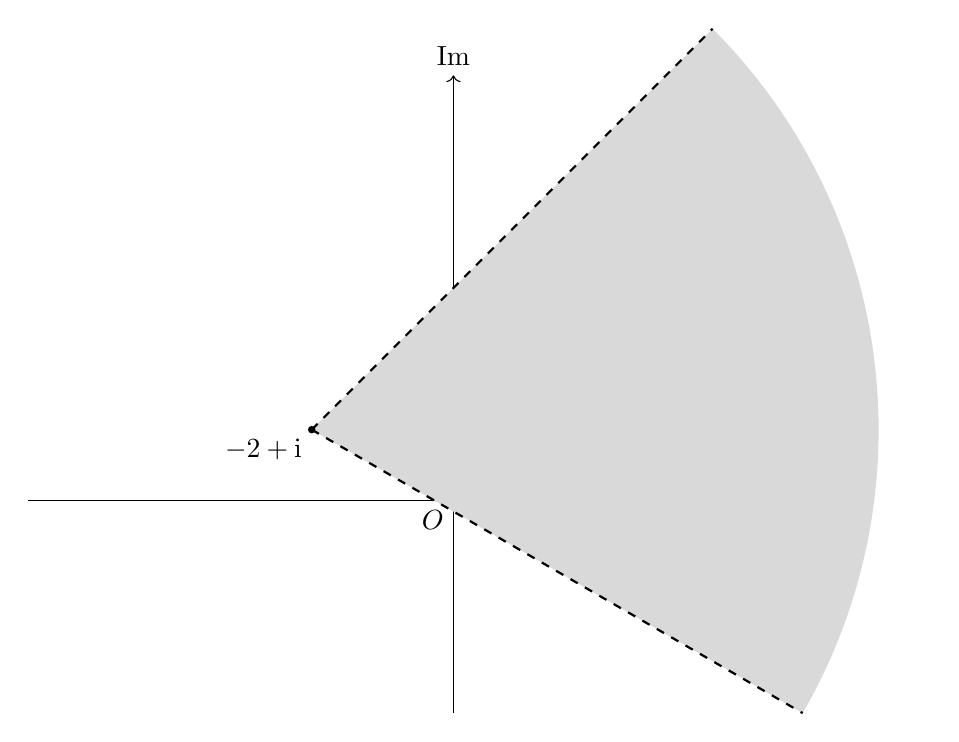
\begin{tikzpicture}[scale=0.9]
      \def\cx{-2}
      \def\cy{1}
      \def\R{8}
      \draw[->] (-6,0) -- (4.5,0) node[right] {Re};
      \draw[->] (0,-3) -- (0,6) node[above] {Im};
      \node[below left] at (0,0) {$O$};
      \fill[gray!30] (\cx,\cy) -- ++(-30:\R) arc (-30:45:\R) -- cycle;
      \draw[thick,dashed] (\cx,\cy) -- ++(-30:\R);
      \draw[thick,dashed] (\cx,\cy) -- ++(45:\R);
      \fill (\cx,\cy) circle (1.5pt);
      \node[below left] at (\cx,\cy) {$-2+\mathrm{i}$};
    \end{tikzpicture}

    \item For the point $z=1+5\mathrm{i}$,
    \[
    z+2-\mathrm{i}=(1+5\mathrm{i})+2-\mathrm{i}=3+4\mathrm{i}
    \]

    So
    \[
    \arg(z+2-\mathrm{i})=\arg(3+4\mathrm{i})=\tan^{-1}\!\left(\frac{4}{3}\right)\approx 0.927
    \]

    But
    \[
    \frac{\pi}{4}\approx 0.785
    \]

    Since
    \[
    0.927>\frac{\pi}{4}
    \]
    the argument is too large, so $1+5\mathrm{i}$ does not lie in the region.

    Therefore, the point $1+5\mathrm{i}$ is not in the region.
  \end{enumerate}
\end{enumerate}
\end{tcolorbox}


\newpage

% ---- Question 5 ----
\questionitem

\begin{figure}[H]
    \centering
\begin{tikzpicture}[scale=1]
\coordinate (O) at (0,0);
\draw[thick, -{Stealth[length=3mm]}] (-2.8,0) -- (6.8,0) node[right] {$\mathrm{Re}(z)$};
\draw[thick, -{Stealth[length=3mm]}] (0,-5.8) -- (0,3.8) node[above] {$\mathrm{Im}(z)$};
\node[below left] at (O) {$O$};
\end{tikzpicture}
\end{figure}


\begin{enumerate}[label=\textbf{(\alph*)}]
  \item Find the modulus of the complex number $2+2\sqrt{3}\mathrm{i}$, giving your answer as an integer. \marks{2} \\
  \item The locus of points, $L$, satisfies the equation $|z-(2-2\sqrt{3}\mathrm{i})|=2$.
  \begin{enumerate}[label=(\roman*)]
    \item Sketch the locus $L$ on the Argand diagram below. \marks{3}
    \item The complex number $w$ lies on $L$ so that $-\pi<\arg w\leq \pi$. Find the greatest possible value of $\arg w$, giving your answer in terms of $\pi$. \marks{2} \\
  \end{enumerate}
  \item Solve the equation $z^4=2+2\sqrt{3}\mathrm{i}$, giving your answers in the form $re^{\mathrm{i}\theta}$, where $r>0$ and $-\pi<\theta\leq \pi$. \marks{5} \\
\end{enumerate}

\vspace*{10pt}

\begin{tcolorbox}[colback=white, colframe=scarlet, title={\textbf{Solution}}, breakable, grow to left by=6mm, grow to right by=10mm]
\begin{enumerate}[label=\textbf{(\alph*)}]
  \item The modulus is
  \[
  \lvert 2+2\sqrt{3}\mathrm{i}\rvert=\sqrt{2^2+(2\sqrt{3})^2}
  =\sqrt{4+12}
  =\sqrt{16}
  =4
  \]
  So the modulus is \(4\).

  \item \begin{enumerate}[label=\textbf{(\roman*)}]
    \item The equation
    \[
    \lvert z-(2-2\sqrt{3}\mathrm{i})\rvert=2
    \]
    represents all points a distance \(2\) from the point \(2-2\sqrt{3}\mathrm{i}\).

    So \(L\) is a circle with centre \((2,-2\sqrt{3})\) and radius \(2\).


    \begin{figure}[H]
    \centering
\begin{tikzpicture}[scale=0.8]
\coordinate (O) at (0,0);
\coordinate (C) at (2,-3.464101615);   % (2,-2sqrt3)
\coordinate (W) at (3,-1.732050808);   % (3,-sqrt3)

\draw[thick, -{Stealth[length=3mm]}] (-2.8,0) -- (6.8,0) node[right] {$\mathrm{Re}(z)$};
\draw[thick, -{Stealth[length=3mm]}] (0,-5.8) -- (0,3.8) node[above] {$\mathrm{Im}(z)$};

\draw[thick] (C) circle (2);

\fill (C) circle (2pt);

\draw[thick] (2,0.12) -- (2,-0.12);
\draw[thick] (0.12,-3.464101615) -- (-0.12,-3.464101615);

\node[below left] at (O) {$O$};
\node[below] at (2,0) {$2$};
\node[left] at (0,-3.464101615) {$-2\sqrt{3}$};

\node[right] at (C) {$2-2\sqrt{3}\mathrm{i}$};
\node[above right] at (4,-2.5) {$L$};

\end{tikzpicture}
\end{figure}

    \item Let \(C\) be the centre of the circle, so
    \[
    C=2-2\sqrt{3}\mathrm{i}
    \]

    First find \(OC\):
    \[
    OC=\lvert 2-2\sqrt{3}\mathrm{i}\rvert
    =\sqrt{2^2+(-2\sqrt{3})^2}
    =\sqrt{4+12}
    =4
    \]

    Also,
    \[
    \arg C=-\frac{\pi}{3}
    \]
    because \(C\) is in the fourth quadrant and
    \[
    \tan |\arg C|=\frac{2\sqrt{3}}{2}=\sqrt{3}
    \]

    The greatest possible value of \(\arg w\) occurs when the line from the origin to the circle is a tangent, touching the circle at \(w\).


    \begin{figure}[H]
    \centering
\begin{tikzpicture}[scale=0.8]
\coordinate (O) at (0,0);
\coordinate (C) at (2,-3.464101615);   % (2,-2sqrt3)
\coordinate (W) at (3,-1.732050808);   % (3,-sqrt3)

\draw[thick, -{Stealth[length=3mm]}] (-2.8,0) -- (6.8,0) node[right] {$\mathrm{Re}(z)$};
\draw[thick, -{Stealth[length=3mm]}] (0,-5.8) -- (0,3.8) node[above] {$\mathrm{Im}(z)$};

\draw[thick] (C) circle (2);

\draw[thick] (O) -- (W);
\draw[dashed] (O) -- (C);
\draw[dashed] (C) -- (W);

\fill (C) circle (2pt);
\fill (W) circle (2pt);

\draw[thick] (2,0.12) -- (2,-0.12);
\draw[thick] (0.12,-3.464101615) -- (-0.12,-3.464101615);

\node[below left] at (O) {$O$};
\node[below] at (2,0) {$2$};
\node[left] at (0,-3.464101615) {$-2\sqrt{3}$};

\node[right] at (C) {$2-2\sqrt{3}\mathrm{i}$};
\node[above right] at (W) {$w$};
\node[above right] at (4,-2.5) {$L$};

\draw[thick] ($(W)+(-0.18,0.10)$) -- ($(W)+(-0.28,-0.07)$) -- ($(W)+(-0.10,-0.17)$);

\node at (1.15,-0.42) {$-\frac{\pi}{6}$};
\end{tikzpicture}
\end{figure}

    Then triangle \(OCW\) is right-angled at \(W\), with
    \[
    CW=2,\qquad OC=4
    \]

    Let \(\angle COW=\alpha\). Then
    \[
    \sin\alpha=\frac{CW}{OC}=\frac{2}{4}=\frac{1}{2}
    \]
    so
    \[
    \alpha=\frac{\pi}{6}
    \]

    Since this tangent is above the line \(OC\),
    \[
    \arg w=\arg C+\alpha=-\frac{\pi}{3}+\frac{\pi}{6}=-\frac{\pi}{6}
    \]

    Therefore the greatest possible value of \(\arg w\) is \(-\dfrac{\pi}{6}\).
  \end{enumerate}

  \item From part (a),
  \[
  \lvert 2+2\sqrt{3}\mathrm{i}\rvert=4
  \]
  and since \(2+2\sqrt{3}\mathrm{i}\) lies in the first quadrant,
  \[
  \arg(2+2\sqrt{3}\mathrm{i})=\frac{\pi}{3}
  \]

  So
  \[
  2+2\sqrt{3}\mathrm{i}=4e^{\mathrm{i}\pi/3}
  \]

  We solve
  \[
  z^4=4e^{\mathrm{i}\pi/3}
  \]

  Let \(z=re^{\mathrm{i}\theta}\). Then
  \[
  z^4=r^4e^{\mathrm{i}4\theta}
  \]
  so
  \[
  r^4e^{\mathrm{i}4\theta}=4e^{\mathrm{i}(\pi/3+2k\pi)}
  \qquad (k\in\mathbb{Z})
  \]

  Equating moduli gives
  \[
  r^4=4
  \]
  so, with \(r>0\),
  \[
  r=4^{1/4}=\sqrt{2}
  \]

  Equating arguments gives
  \[
  4\theta=\frac{\pi}{3}+2k\pi
  \]
  hence
  \[
  \theta=\frac{\pi}{12}+\frac{k\pi}{2}
  \]

  The four distinct roots come from \(k=0,1,2,3\):
  \[
  \theta=\frac{\pi}{12},\quad \frac{7\pi}{12},\quad \frac{13\pi}{12},\quad \frac{19\pi}{12}
  \]

  Writing these in the range \(-\pi<\theta\leq\pi\),
  \[
  \theta=\frac{\pi}{12},\quad \frac{7\pi}{12},\quad -\frac{11\pi}{12},\quad -\frac{5\pi}{12}
  \]

  Therefore
  \[
  z=\sqrt{2}e^{\mathrm{i}\pi/12},\qquad
  \sqrt{2}e^{\mathrm{i}7\pi/12},\qquad
  \sqrt{2}e^{-\mathrm{i}11\pi/12},\qquad
  \sqrt{2}e^{-\mathrm{i}5\pi/12}
  \]

  These are the four solutions.
\end{enumerate}
\end{tcolorbox}


\newpage

% ---- Question 6 ----
\questionitem

The point $P$ represents a complex number $z$ on an Argand diagram such that
\[
|z-(1+\mathrm{i})|=\frac{1}{2}|z-(4+\mathrm{i})|
\] \\

\begin{enumerate}[label=\textbf{(\alph*)}]
  \item Show that, as $z$ varies, the locus of $P$ is a circle, and give the coordinates of the centre and the radius of the circle. \marks{5} \\
\end{enumerate}

The point $Q$ represents a complex number $z$ on an Argand diagram such that
\[
|z-(2+3\mathrm{i})|=|z+2-\mathrm{i}|
\] \\

\begin{enumerate}[label=\textbf{(\alph*)}, resume]
  \item Sketch, on the same Argand diagram, the locus of $P$ and the locus of $Q$ as $z$ varies. \marks{5} \\
  \item On your diagram shade the region which satisfies
  \[
  |z-(1+\mathrm{i})|\le \frac{1}{2}|z-(4+\mathrm{i})| \quad \text{and} \quad |z-(2+3\mathrm{i})|\ge |z+2-\mathrm{i}|
  \]
  \marks[-20pt]{2}
\end{enumerate}

\vspace*{10pt}

\begin{tcolorbox}[colback=white, colframe=scarlet, title={\textbf{Solution}}, breakable, grow to left by=6mm, grow to right by=10mm]
\begin{enumerate}[label=\textbf{(\alph*)}]
  \item Let
  \[
  z=x+\mathrm{i}y
  \]
  Then
  \[
  \lvert z-(1+\mathrm{i})\rvert=\sqrt{(x-1)^2+(y-1)^2}
  \]
  and
  \[
  \lvert z-(4+\mathrm{i})\rvert=\sqrt{(x-4)^2+(y-1)^2}
  \]

  So the given condition becomes
  \[
  \sqrt{(x-1)^2+(y-1)^2}=\frac12\sqrt{(x-4)^2+(y-1)^2}
  \]

  Squaring both sides,
  \[
  4\bigl((x-1)^2+(y-1)^2\bigr)=(x-4)^2+(y-1)^2
  \]

  Expand:
  \begin{align*}
  4\bigl(x^2-2x+1+y^2-2y+1\bigr)&=x^2-8x+16+y^2-2y+1\\
  4x^2-8x+4+4y^2-8y+4&=x^2-8x+16+y^2-2y+1
  \end{align*}

  Bring everything to one side:
  \begin{align*}
  3x^2+3y^2-6y-9&=0\\
  x^2+y^2-2y-3&=0
  \end{align*}

  Complete the square in $y$:
  \begin{align*}
  x^2+(y^2-2y+1)-4&=0\\
  x^2+(y-1)^2&=4
  \end{align*}

  This is the equation of a circle.

  Hence the locus is the circle with centre $(0,1)$ and radius $2$.

  \item For the second locus, let again $z=x+\mathrm{i}y$.

  Then
  \[
  \lvert z-(2+3\mathrm{i})\rvert=\sqrt{(x-2)^2+(y-3)^2}
  \]
  and
  \[
  \lvert z+2-\mathrm{i}\rvert=\lvert z-(-2+\mathrm{i})\rvert=\sqrt{(x+2)^2+(y-1)^2}
  \]

  So
  \[
  \sqrt{(x-2)^2+(y-3)^2}=\sqrt{(x+2)^2+(y-1)^2}
  \]

  Squaring both sides,
  \[
  (x-2)^2+(y-3)^2=(x+2)^2+(y-1)^2
  \]

  Expand and simplify:
  \begin{align*}
  x^2-4x+4+y^2-6y+9&=x^2+4x+4+y^2-2y+1\\
  -4x-6y+13&=4x-2y+5\\
  -8x-4y+8&=0\\
  2x+y-2&=0
  \end{align*}

  So the locus of $Q$ is the straight line
  \[
  y=2-2x
  \]

  This is the perpendicular bisector of the line segment joining $(2,3)$ and $(-2,1)$.

  On the same Argand diagram, we sketch:
  \begin{itemize}
    \item the circle $x^2+(y-1)^2=4$, centre $(0,1)$, radius $2$,
    \item the line $y=2-2x$.
  \end{itemize}

  \begin{center}
  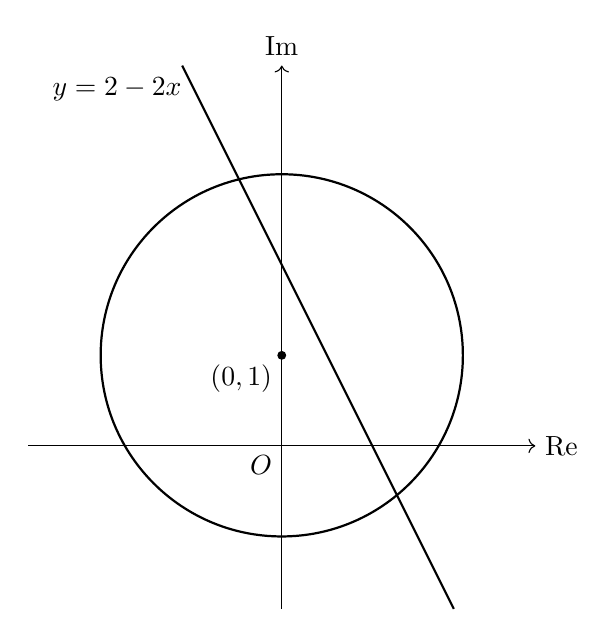
\begin{tikzpicture}[scale=1.15]
  \def\cx{0}
  \def\cy{1}
  \def\rad{2}
  \draw[->] (-2.8,0) -- (2.8,0) node[right] {Re};
  \draw[->] (0,-1.8) -- (0,4.2) node[above] {Im};
  \node[below left] at (0,0) {$O$};

  \draw[thick] (\cx,\cy) circle (\rad);
  \draw[thick] (-1.1,4.2) -- (1.9,-1.8);

  \fill (\cx,\cy) circle (1.4pt);
  \node[below left] at (\cx,\cy) {$(0,1)$};
  \node[above left] at (-1.0,3.7) {$y=2-2x$};
  \end{tikzpicture}
  \end{center}

  \item From part (a),
  \[
  \lvert z-(1+\mathrm{i})\rvert\le \frac12\lvert z-(4+\mathrm{i})\rvert
  \]
  gives
  \[
  x^2+(y-1)^2\le 4
  \]
  so the point lies inside or on the circle.

  From part (b),
  \[
  \lvert z-(2+3\mathrm{i})\rvert\ge \lvert z+2-\mathrm{i}\rvert
  \]
  gives
  \begin{align*}
  (x-2)^2+(y-3)^2&\ge (x+2)^2+(y-1)^2\\
  -8x-4y+8&\ge 0\\
  2x+y-2&\le 0\\
  y&\le 2-2x
  \end{align*}

  So the point lies on or below the line $y=2-2x$.

  Therefore the required region is the intersection of:
  \begin{itemize}
    \item the inside of the circle $x^2+(y-1)^2=4$,
    \item the half-plane $y\le 2-2x$.
  \end{itemize}

  The shaded region is shown below.

  \begin{center}
  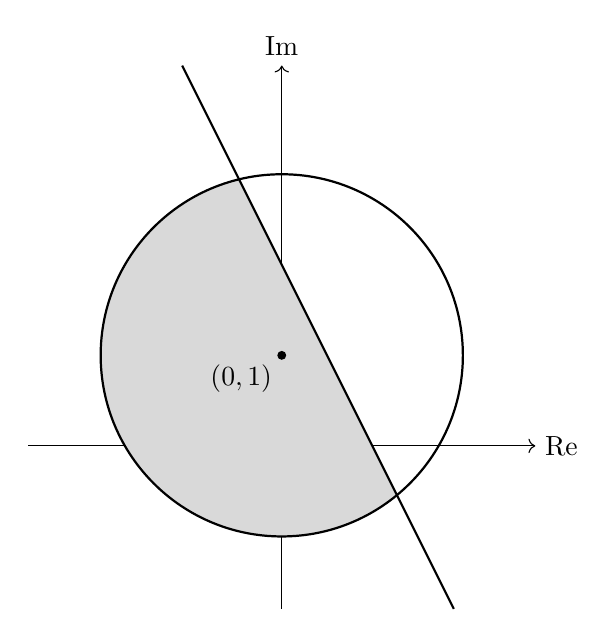
\begin{tikzpicture}[scale=1.15]
  \def\cx{0}
  \def\cy{1}
  \def\rad{2}

  \draw[->] (-2.8,0) -- (2.8,0) node[right] {Re};
  \draw[->] (0,-1.8) -- (0,4.2) node[above] {Im};
  \node[below left] at (0,0) {$O$};

  \begin{scope}
    \clip (\cx,\cy) circle (\rad);
    \fill[gray!30] (-3,-2) -- (2,-2) -- (-1,4) -- (-3,4) -- cycle;
  \end{scope}

  \draw[thick] (\cx,\cy) circle (\rad);
  \draw[thick] (-1.1,4.2) -- (1.9,-1.8);

  \fill (\cx,\cy) circle (1.4pt);
  \node[below left] at (\cx,\cy) {$(0,1)$};
  \end{tikzpicture}
  \end{center}

  So the region is inside the circle and on/below the line.
\end{enumerate}
\end{tcolorbox}


\newpage

% ---- Question 7 ----
\questionitem

On an Argand diagram, the point $P$ representing the complex number $z$ lies on the locus
\[
\lvert z-(2-\mathrm{i})\rvert =3
\]
The point $Q$ representing the complex number $w$ lies on the locus
\[
\lvert w+1-11\mathrm{i}\rvert =3\lvert w+1-3\mathrm{i}\rvert
\]
Find the exact coordinates of the points common to these two loci. \marks{7}

\vspace*{10pt}

\begin{tcolorbox}[colback=white, colframe=scarlet, title={\textbf{Solution}}, breakable, grow to left by=6mm, grow to right by=10mm]
Let a point common to both loci have affix
\[
u=x+y\mathrm{i}
\]
so its coordinates are \((x,y)\).

For the locus of \(P\),
\[
|u-(2-\mathrm{i})|=3
\]
Now
\[
u-(2-\mathrm{i})=(x-2)+(y+1)\mathrm{i}
\]
so
\[
|(x-2)+(y+1)\mathrm{i}|=3
\]
Using \(|a+b\mathrm{i}|=\sqrt{a^2+b^2}\),
\[
(x-2)^2+(y+1)^2=9
\]

For the locus of \(Q\),
\[
|u+1-11\mathrm{i}|=3|u+1-3\mathrm{i}|
\]
Now
\[
u+1-11\mathrm{i}=(x+1)+(y-11)\mathrm{i},\qquad
u+1-3\mathrm{i}=(x+1)+(y-3)\mathrm{i}
\]
So
\[
|(x+1)+(y-11)\mathrm{i}|=3|(x+1)+(y-3)\mathrm{i}|
\]
Squaring both sides gives
\[
(x+1)^2+(y-11)^2=9\bigl((x+1)^2+(y-3)^2\bigr)
\]
Expand and simplify:
\begin{align*}
x^2+2x+1+y^2-22y+121 &= 9x^2+18x+9+9y^2-54y+81 \\
0 &= 8x^2+16x+8+8y^2-32y-32 \\
0 &= x^2+2x+y^2-4y-4 \\
0 &= (x+1)^2+(y-2)^2-9
\end{align*}
Hence the second locus is
\[
(x+1)^2+(y-2)^2=9
\]

So the common points satisfy the simultaneous equations
\[
(x-2)^2+(y+1)^2=9
\]
and
\[
(x+1)^2+(y-2)^2=9
\]

Subtracting one equation from the other:
\begin{align*}
(x-2)^2+(y+1)^2 &= (x+1)^2+(y-2)^2 \\
x^2-4x+4+y^2+2y+1 &= x^2+2x+1+y^2-4y+4 \\
-6x+6y &= 0 \\
y&=x
\end{align*}

Substitute \(y=x\) into \((x-2)^2+(y+1)^2=9\):
\begin{align*}
(x-2)^2+(x+1)^2 &= 9 \\
x^2-4x+4+x^2+2x+1 &= 9 \\
2x^2-2x-4 &= 0 \\
x^2-x-2 &= 0 \\
(x-2)(x+1) &= 0
\end{align*}
So
\[
x=2 \quad \text{or} \quad x=-1
\]
and since \(y=x\),
\[
y=2 \quad \text{or} \quad y=-1
\]

Therefore the exact coordinates of the common points are
\[
(2,2)\quad \text{and}\quad (-1,-1)
\]
\end{tcolorbox}


\newpage

% ---- Question 8 ----
\questionitem

\begin{figure}[H]
    \centering
\begin{tikzpicture}[scale=0.9]
\draw[->, thick] (-2.2,0) -- (6.7,0) node[right] {$\mathrm{Re}(z)$};
\draw[->, thick] (0,-2.2) -- (0,5.7) node[above] {$\mathrm{Im}(z)$};
\foreach \x in {-2,-1,1,2,3,4,5,6} {
  \draw (\x,0.12) -- (\x,-0.12) node[below] {$\x$};
}
\foreach \y in {-2,-1,1,2,3,4,5} {
  \draw (0.12,\y) -- (-0.12,\y) node[left] {$\y$};
}
\node[below left] at (0,0) {$O$};
\end{tikzpicture}
\end{figure}


\begin{enumerate}[label=\textbf{(\alph*)}]
  \item Sketch, on the Argand diagram below, the locus of points satisfying the equation
  \[
  |z-(3+\mathrm{i})|=1
  \]
  \marks[-20pt]{1}
  \item There is a unique complex number $w$ that satisfies both
  \[
  |w-(3+\mathrm{i})|=1 \quad \text{and} \quad \arg(w)=\alpha
  \]
  where $\alpha$ is a constant such that $0<\alpha<\pi$.
  \begin{enumerate}[label=(\roman*)]
    \item Find the value of $\alpha$. \marks{2}
    \item Find $w$ and express it in the form $r(\cos\theta+\mathrm{i}\sin\theta)$. Give each of $r$ and $\theta$ to two significant figures. \marks{4} \\
  \end{enumerate}
\end{enumerate}

\vspace*{0pt}

\begin{tcolorbox}[colback=white, colframe=scarlet, title={\textbf{Solution}}, breakable, grow to left by=6mm, grow to right by=10mm]
\begin{enumerate}[label=\textbf{(\alph*)}]
  \item The locus
  \[
  |z-(3+\mathrm{i})|=1
  \]
  is the set of points whose distance from \(3+\mathrm{i}\) is \(1\).

  So it is a circle with centre \((3,1)\) and radius \(1\).

  
\begin{figure}[H]
    \centering
\begin{tikzpicture}[scale=1]
    \def\cx{3}
    \def\cy{1}
    \def\rad{1}
\draw[->, thick] (-2.2,0) -- (6.7,0) node[right] {$\mathrm{Re}(z)$};
\draw[->, thick] (0,-2.2) -- (0,5.7) node[above] {$\mathrm{Im}(z)$};
\foreach \x in {-2,-1,1,2,3,4,5,6} {
  \draw (\x,0.12) -- (\x,-0.12) node[below] {$\x$};
}
\foreach \y in {-2,-1,1,2,3,4,5} {
  \draw (0.12,\y) -- (-0.12,\y) node[left] {$\y$};
}
    \draw[thick] (\cx,\cy) circle (\rad);
    \fill (\cx,\cy) circle (1.5pt);
    \node[above right] at (\cx,\cy) {$3+\mathrm{i}$};
\node[below left] at (0,0) {$O$};
\end{tikzpicture}
\end{figure}

  \item
  \begin{enumerate}[label=(\roman*)]
    \item If \(\arg(w)=\alpha\), then \(w\) lies on a straight line through the origin, so its equation is
    \[
    y=mx
    \]
    where
    \[
    m=\tan\alpha
    \]

    For there to be a unique point \(w\) satisfying both conditions, this line must touch the circle at exactly one point, so it must be a tangent.

    The circle has centre \((3,1)\) and radius \(1\).  
    The distance from \((3,1)\) to the line \(y=mx\), written as \(mx-y=0\), is
    \[
    \frac{|3m-1|}{\sqrt{m^2+1}}
    \]

    Since this distance equals the radius,
    \[
    \frac{|3m-1|}{\sqrt{m^2+1}}=1
    \]

    Squaring both sides,
    \begin{align*}
    (3m-1)^2 &= m^2+1 \\
    9m^2-6m+1 &= m^2+1 \\
    8m^2-6m &= 0 \\
    2m(4m-3) &= 0
    \end{align*}

    So
    \[
    m=0 \quad \text{or} \quad m=\frac34
    \]

    If \(m=0\), then \(\alpha=0\), but the question states \(0<\alpha<\pi\), so this is not allowed.

    Hence
    \[
    \tan\alpha=\frac34
    \]
    so
    \[
    \alpha=\arctan\!\left(\frac34\right)\approx 0.64
    \]

    Therefore, \(\alpha=\arctan\!\left(\frac34\right)\approx 0.64\) rad.

    \item Using the value of \(m\), the tangent line is
    \[
    y=\frac34x
    \]

    The circle equation is
    \[
    (x-3)^2+(y-1)^2=1
    \]

    Substituting \(y=\frac34x\),
    \begin{align*}
    (x-3)^2+\left(\frac34x-1\right)^2 &= 1 \\
    x^2-6x+9+\frac{9}{16}x^2-\frac32x+1 &= 1 \\
    \frac{25}{16}x^2-\frac{15}{2}x+9 &= 0
    \end{align*}

    Multiplying by \(16\),
    \[
    25x^2-120x+144=0
    \]

    Factorising,
    \[
    (5x-12)^2=0
    \]

    So
    \[
    x=\frac{12}{5}
    \]

    Then
    \[
    y=\frac34\cdot\frac{12}{5}=\frac{9}{5}
    \]

    Hence
    \[
    w=\frac{12}{5}+\frac{9}{5}\mathrm{i}
    \]

    Now find its modulus:
    \begin{align*}
    |w| &= \sqrt{\left(\frac{12}{5}\right)^2+\left(\frac{9}{5}\right)^2} \\
        &= \sqrt{\frac{144}{25}+\frac{81}{25}} \\
        &= \sqrt{\frac{225}{25}} \\
        &= 3
    \end{align*}

    Its argument is
    \[
    \theta=\arg(w)=\alpha=\arctan\!\left(\frac34\right)\approx 0.64
    \]

    So in modulus-argument form,
    \[
    w=3(\cos 0.64+\mathrm{i}\sin 0.64)
    \]

    To two significant figures,
    \[
    r=3.0,\qquad \theta=0.64
    \]

    Therefore,
    \[
    w=\frac{12}{5}+\frac{9}{5}\mathrm{i}=3(\cos 0.64+\mathrm{i}\sin 0.64)
    \]
  \end{enumerate}
\end{enumerate}
\end{tcolorbox}


\newpage

% ---- Question 9 ----
\questionitem

The locus of points $z=x+\mathrm{i}y$ that satisfy
\[
\arg\left(\frac{z-(2+\mathrm{i})}{z-(6+5\mathrm{i})}\right)=\frac{\pi}{4}
\]
is an arc of a circle $C$. \\

\begin{enumerate}[label=\textbf{(\alph*)}]
  \item On an Argand diagram sketch the locus of $z$. \marks{2} \\
  \item Explain why the centre of $C$ lies on the line $y=7-x$. \marks{1} \\
  \item Determine the radius of $C$. \marks{2} \\
  \item Determine the coordinates of the centre of $C$. \marks{2} \\
\end{enumerate}

\vspace*{10pt}

\begin{tcolorbox}[colback=white, colframe=scarlet, title={\textbf{Solution}}, breakable, grow to left by=6mm, grow to right by=10mm]
\begin{enumerate}[label=\textbf{(\alph*)}]
  \item Let
  \[
  A=2+\mathrm{i}\quad\text{and}\quad B=6+5\mathrm{i}
  \]
  so \(A=(2,1)\) and \(B=(6,5)\).

  The condition
  \[
  \arg\left(\frac{z-A}{z-B}\right)=\frac{\pi}{4}
  \]
  means
  \[
  \arg(z-A)-\arg(z-B)=\frac{\pi}{4}
  \]
  so the angle between the lines \(ZA\) and \(ZB\) is \(\frac{\pi}{4}\).

  Hence the locus is an arc of a circle through \(A\) and \(B\), and the required arc is the one on the side below/right of the line segment \(AB\). Also, \(A\) and \(B\) are excluded because the expression is undefined there.

  \[
  \begin{tikzpicture}[scale=0.75]
    \draw[->] (-0.5,0) -- (11,0) node[right] {Re};
    \draw[->] (0,-3.5) -- (0,6.5) node[above] {Im};
    \node[below left] at (0,0) {$O$};

    \draw[dashed] (2,1) -- (6,5);

    \draw[thick] (2,1) arc[start angle=180, end angle=450, radius=4];

    \draw[fill=white] (2,1) circle (2pt);
    \draw[fill=white] (6,5) circle (2pt);

    \node[below left] at (2,1) {$A(2,1)$};
    \node[above right] at (6,5) {$B(6,5)$};
  \end{tikzpicture}
  \]

  So the sketch is the arc through \((2,1)\) and \((6,5)\) on the side below/right of \(AB\), with endpoints excluded.

  \item Since \(A\) and \(B\) lie on circle \(C\), the centre of \(C\) is equidistant from \(A\) and \(B\). Therefore it lies on the perpendicular bisector of \(AB\).

  The midpoint of \(AB\) is
  \[
  \left(\frac{2+6}{2},\frac{1+5}{2}\right)=(4,3)
  \]

  The slope of \(AB\) is
  \[
  \frac{5-1}{6-2}=1
  \]
  so the perpendicular bisector has slope \(-1\).

  Its equation is
  \[
  y-3=-1(x-4)
  \]
  \[
  y=7-x
  \]

  Therefore the centre lies on the line \(y=7-x\).

  \item First find the length of chord \(AB\):
  \[
  |AB|=\sqrt{(6-2)^2+(5-1)^2}
  \]
  \[
  |AB|=\sqrt{4^2+4^2}=\sqrt{32}=4\sqrt{2}
  \]

  The angle at the circumference is \(\frac{\pi}{4}\), so the angle at the centre subtended by the same chord is
  \[
  2\times \frac{\pi}{4}=\frac{\pi}{2}
  \]

  If the radius is \(r\), then using the chord formula
  \[
  |AB|=2r\sin\left(\frac{1}{2}\times \frac{\pi}{2}\right)
  \]
  \[
  4\sqrt{2}=2r\sin\frac{\pi}{4}=2r\cdot\frac{\sqrt{2}}{2}=r\sqrt{2}
  \]

  So
  \[
  r=4
  \]

  Therefore the radius of \(C\) is \(4\).

  \item Let \(M\) be the midpoint of \(AB\), so \(M=(4,3)\).

  From part (b), the centre lies on \(y=7-x\), and from part (c) the radius is \(4\).

  Also,
  \[
  \frac{|AB|}{2}=2\sqrt{2}
  \]

  In the right-angled triangle formed by the centre, the midpoint of the chord, and one end of the chord,
  \[
  OM=\sqrt{r^2-\left(\frac{|AB|}{2}\right)^2}
  \]
  \[
  OM=\sqrt{4^2-(2\sqrt{2})^2}
  =\sqrt{16-8}
  =\sqrt{8}
  =2\sqrt{2}
  \]

  The line \(y=7-x\) has direction vector
  \[
  \begin{pmatrix}1\\-1\end{pmatrix}
  \]
  which has length \(\sqrt{2}\). So moving a distance \(2\sqrt{2}\) along this line means moving by
  \[
  \pm 2\begin{pmatrix}1\\-1\end{pmatrix}
  \]

  Hence the two possible centres are
  \[
  (4,3)+(2,-2)=(6,1)
  \]
  and
  \[
  (4,3)+(-2,2)=(2,5)
  \]

  To decide which is correct, test a point on the locus. Take \(z=10+\mathrm{i}\):
  \begin{align*}
  \arg\left(\frac{(10+\mathrm{i})-(2+\mathrm{i})}{(10+\mathrm{i})-(6+5\mathrm{i})}\right)
  &=\arg\left(\frac{8}{4-4\mathrm{i}}\right)\\
  &=\arg\left(\frac{8(4+4\mathrm{i})}{(4-4\mathrm{i})(4+4\mathrm{i})}\right)\\
  &=\arg(1+\mathrm{i})\\
  &=\frac{\pi}{4}
  \end{align*}

  So \(10+\mathrm{i}\) lies on the locus.

  Now check which circle it lies on:
  \[
  \text{distance from }(10,1)\text{ to }(6,1)=4
  \]
  so it lies on the circle centred at \((6,1)\).

  But
  \[
  \text{distance from }(10,1)\text{ to }(2,5)=\sqrt{(8)^2+(-4)^2}=\sqrt{80}\ne 4
  \]
  so it does not lie on the circle centred at \((2,5)\).

  Therefore the centre of \(C\) is \((6,1)\).
\end{enumerate}
\end{tcolorbox}


\newpage

% ---- Question 10 ----
\questionitem

\begin{figure}[H]
    \centering
\begin{tikzpicture}[scale=0.9]
\draw[-{Stealth[length=3mm]}, thick] (-2.2,0) -- (7.7,0) node[right] {$\mathrm{Re}(z)$};
\draw[-{Stealth[length=3mm]}, thick] (0,-1.2) -- (0,7.7) node[above] {$\mathrm{Im}(z)$};

\foreach \x in {-2,-1,1,2,3,4,5,6,7} {
  \draw (\x,0.12) -- (\x,-0.12);
  \node[below] at (\x,-0.12) {$\x$};
}
\foreach \y in {-1,1,2,3,4,5,6,7} {
  \draw (0.12,\y) -- (-0.12,\y);
  \node[left] at (-0.12,\y) {$\y$};
}

\node[below left] at (0,0) {$O$};
\end{tikzpicture}
\end{figure}


\begin{enumerate}[label=\textbf{(\alph*)}]
  \item Sketch, on the Argand diagram below, the locus of points satisfying the equation
  \[
  |z-(2+4\mathrm{i})|=3
  \]
  \marks[-20pt]{2}
  \item Sketch, also on the Argand diagram, the locus of points satisfying the equation
  \[
  \arg(z-1)=\frac{\pi}{4}
  \]
  \marks[-20pt]{1}
  \item For the complex number $w$, find the maximum value of $|w|$ such that
  \[
  |w-(2+4\mathrm{i})|\le 3 \qquad \text{and} \qquad 0\le \arg(w-1)\le \frac{\pi}{4}
  \]
  \marks[-20pt]{3}
\end{enumerate}

\vspace*{5pt}

\begin{tcolorbox}[colback=white, colframe=scarlet, title={\textbf{Solution}}, breakable, grow to left by=6mm, grow to right by=10mm]
\begin{enumerate}[label=\textbf{(\alph*)}]
  \item The locus
  \[
  |z-(2+4\mathrm{i})|=3
  \]
  is a circle with centre at the point representing $2+4\mathrm{i}$ and radius $3$

  \begin{figure}[H]
    \centering
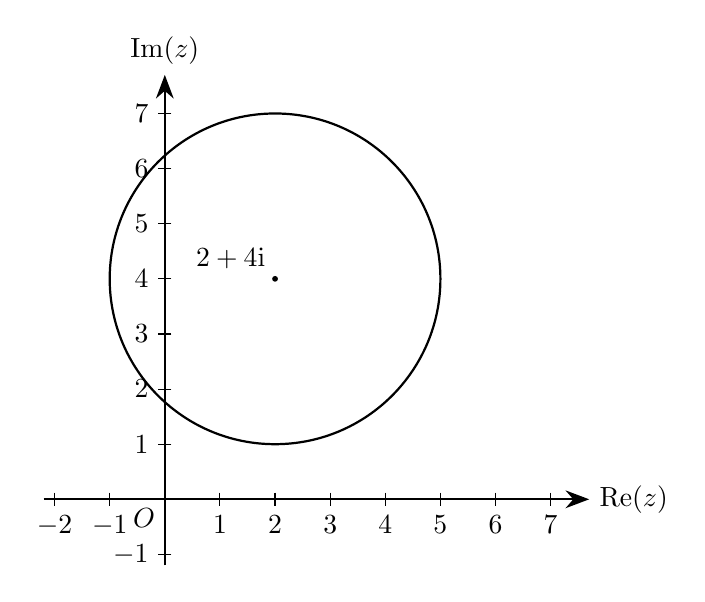
\begin{tikzpicture}[scale=0.7]
\def\cx{2}
\def\cy{4}
\def\rad{3}

\draw[-{Stealth[length=3mm]}, thick] (-2.2,0) -- (7.7,0) node[right] {$\mathrm{Re}(z)$};
\draw[-{Stealth[length=3mm]}, thick] (0,-1.2) -- (0,7.7) node[above] {$\mathrm{Im}(z)$};

\foreach \x in {-2,-1,1,2,3,4,5,6,7} {
  \draw (\x,0.12) -- (\x,-0.12);
  \node[below] at (\x,-0.12) {$\x$};
}
\foreach \y in {-1,1,2,3,4,5,6,7} {
  \draw (0.12,\y) -- (-0.12,\y);
  \node[left] at (-0.12,\y) {$\y$};
}

\node[below left] at (0,0) {$O$};

\draw[thick] (\cx,\cy) circle (\rad);
\fill (\cx,\cy) circle (1.5pt);
\node[above left] at (\cx,\cy) {$2+4\mathrm{i}$};

\end{tikzpicture}
\end{figure}

  \item The locus
  \[
  \arg(z-1)=\frac{\pi}{4}
  \]
  is the half-line starting at the point representing $1$ on the real axis, making an angle of $\frac{\pi}{4}$ with the positive real axis

  In Cartesian form this is
  \[
  y=x-1,\qquad x>1
  \]

\begin{figure}[H]
    \centering
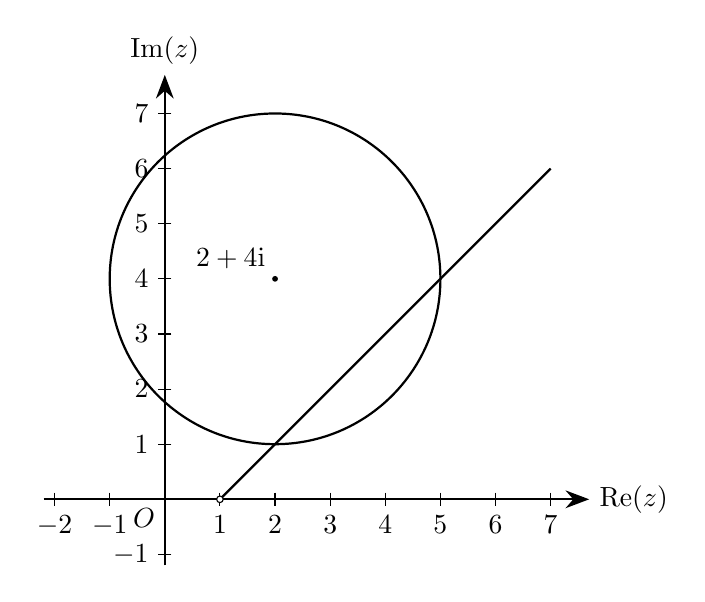
\begin{tikzpicture}[scale=0.7]
\def\cx{2}
\def\cy{4}
\def\rad{3}

\draw[-{Stealth[length=3mm]}, thick] (-2.2,0) -- (7.7,0) node[right] {$\mathrm{Re}(z)$};
\draw[-{Stealth[length=3mm]}, thick] (0,-1.2) -- (0,7.7) node[above] {$\mathrm{Im}(z)$};

\foreach \x in {-2,-1,1,2,3,4,5,6,7} {
  \draw (\x,0.12) -- (\x,-0.12);
  \node[below] at (\x,-0.12) {$\x$};
}
\foreach \y in {-1,1,2,3,4,5,6,7} {
  \draw (0.12,\y) -- (-0.12,\y);
  \node[left] at (-0.12,\y) {$\y$};
}

\node[below left] at (0,0) {$O$};

\draw[thick] (\cx,\cy) circle (\rad);
\fill (\cx,\cy) circle (1.5pt);
\node[above left] at (\cx,\cy) {$2+4\mathrm{i}$};

\draw[thick] (1,0) -- (7,6);
\draw[fill=white] (1,0) circle (1.7pt);

\end{tikzpicture}
\end{figure}

  \item Let
  \[
  w=x+\mathrm{i}y
  \]
  The condition
  \[
  |w-(2+4\mathrm{i})|\leq 3
  \]
  means that $w$ lies inside or on the circle from part (a)

  Also,
  \[
  0\leq \arg(w-1)\leq \frac{\pi}{4}
  \]
  means that $w$ lies in the region from the real axis up to the line $y=x-1$

  \begin{figure}[H]
    \centering
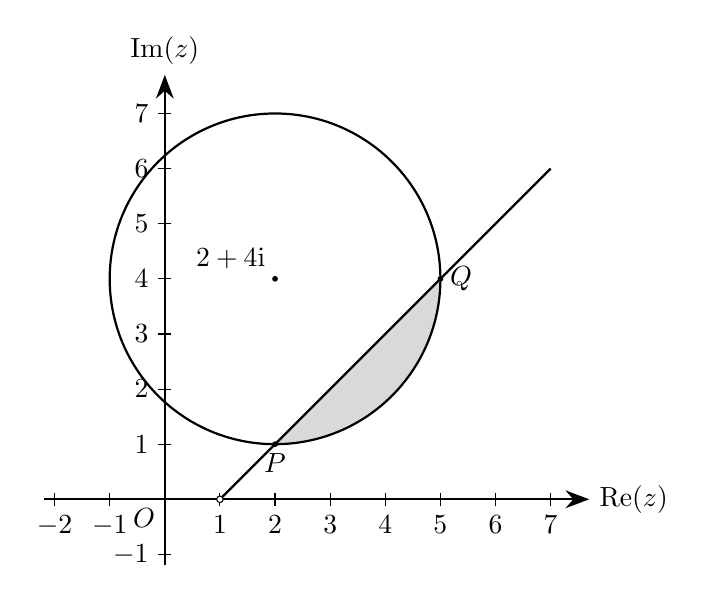
\begin{tikzpicture}[scale=0.7]
\def\cx{2}
\def\cy{4}
\def\rad{3}

\draw[-{Stealth[length=3mm]}, thick] (-2.2,0) -- (7.7,0) node[right] {$\mathrm{Re}(z)$};
\draw[-{Stealth[length=3mm]}, thick] (0,-1.2) -- (0,7.7) node[above] {$\mathrm{Im}(z)$};

\foreach \x in {-2,-1,1,2,3,4,5,6,7} {
  \draw (\x,0.12) -- (\x,-0.12);
  \node[below] at (\x,-0.12) {$\x$};
}
\foreach \y in {-1,1,2,3,4,5,6,7} {
  \draw (0.12,\y) -- (-0.12,\y);
  \node[left] at (-0.12,\y) {$\y$};
}

\node[below left] at (0,0) {$O$};

\begin{scope}
  \clip (\cx,\cy) circle (\rad);
  \fill[gray!30] (-2,-4) -- (8,-4) -- (8,7) -- (-2,-3) -- cycle;
\end{scope}

\draw[thick] (\cx,\cy) circle (\rad);

\draw[thick] (1,0) -- (7,6);
\draw[fill=white] (1,0) circle (1.7pt);

\fill (\cx,\cy) circle (1.5pt);
\node[above left] at (\cx,\cy) {$2+4\mathrm{i}$};

\fill (2,1) circle (1.5pt);
\node[below] at (2,1) {$P$};

\fill (5,4) circle (1.5pt);
\node[right] at (5,4) {$Q$};

\end{tikzpicture}
\end{figure}

  Since the circle has lowest point $(2,1)$, every point in the circle has $y\geq 1$, so the condition $\arg(w-1)\geq 0$ is automatically satisfied

  Therefore the required region is the part of the disc lying on or below the line
  \[
  y=x-1
  \]

  First find where this line meets the circle:
  \begin{align*}
  (x-2)^2+(y-4)^2&=9 \\
  (x-2)^2+(x-1-4)^2&=9 \\
  (x-2)^2+(x-5)^2&=9 \\
  x^2-4x+4+x^2-10x+25&=9 \\
  2x^2-14x+20&=0 \\
  x^2-7x+10&=0 \\
  (x-2)(x-5)&=0
  \end{align*}
  so the intersection points are
  \[
  (2,1)\quad \text{and} \quad (5,4)
  \]

  Now use the circle inequality:
  \begin{align*}
  (x-2)^2+(y-4)^2&\leq 9 \\
  x^2-4x+4+y^2-8y+16&\leq 9 \\
  x^2+y^2&\leq 4x+8y-11
  \end{align*}
  But in the required region, $y\leq x-1$, so
  \begin{align*}
  |w|^2=x^2+y^2&\leq 4x+8y-11 \\
  &\leq 4x+8(x-1)-11 \\
  &=12x-19
  \end{align*}
  Also, inside the circle the greatest possible value of $x$ is $5$, so
  \[
  |w|^2\leq 12(5)-19=41
  \]
  Equality is possible when $x=5$ and $y=x-1=4$, giving
  \[
  w=5+4\mathrm{i}
  \]
  Hence the maximum value of $|w|$ is
  \[
  |w|_{\max}=\sqrt{41}
  \]

  So the maximum value is $\sqrt{41}$, attained when $w=5+4\mathrm{i}$

\end{enumerate}
\end{tcolorbox}


\end{enumerate}
\end{document}
